\chapter{JPEG 图像有损压缩}
\section{颜色空间转换与色度采样}
\subsection{颜色空间转换}

需要将 RGB 颜色空间转化为 YUV 颜色空间,也叫 YCbCr,其中,Y 是亮度 (Luminance),U 和 V 表示色度 (Chrominance) 和浓度 (Chroma),UV 分量同时表示色差

做这一步的原因是对于人眼来说,图像中明暗的变化更容易被感知到,而对颜色的变化则没有那么敏感,将两者分开,就可以根据数据的重要程度的做不同的处理


研究表明,红绿蓝三基色所贡献的亮度不同,绿色所贡献亮度最多,蓝色所贡献亮度最少。假定红色贡献为 $K_R$,蓝色贡献为 $K_B$,则亮度可以表示为
\begin{equation}
    Y = K_R \cdot R + (1-K_R-K_B) \cdot G + K_B \cdot B
\end{equation}

根据经验值 $K_R=0.299, K_B=0.114$,则有
\begin{equation}
    Y = 0.299 \cdot R + 0.587 \cdot G + 0.114 \cdot B
\end{equation}

蓝色和红色的色差为
\begin{equation}
    \begin{aligned}
        Y   &= 0.299   \cdot R + 0.587    \cdot G + 0.114 \cdot B \\
        C_b &= -0.1687 \cdot R - 0.3313   \cdot G + 0.5 \cdot B +128\\
        C_r &= 0.5   \cdot R - 0.4187   \cdot G - 0.0813 \cdot B +128\\
    \end{aligned}    
\end{equation}
或
\begin{equation}
    \begin{bmatrix}
        Y \\ U \\ V
    \end{bmatrix}
    =\begin{bmatrix}
        0.299   & 0.587    & 0.114 & \\
        -0.1687 & -0.3313   & 0.5 & \\
        0.5     & -0.4187   & -0.0813 &
    \end{bmatrix}
    \begin{bmatrix}
        R \\ G \\ B
    \end{bmatrix}
    +\begin{bmatrix}
        0 \\ 128 \\ 128
    \end{bmatrix}
\end{equation}


\subsection{色度采样}
为了进一步压缩图像数据,JPEG对色度图像二次采样。YUV有三种采样方式:

4:4:4采样:每一个Y对应一个U和一个V。

4:2:2采样:每两个Y共用一对U和V。

4:2:0采样:每四个Y共用一对U和V。

\begin{figure}
    \centering
    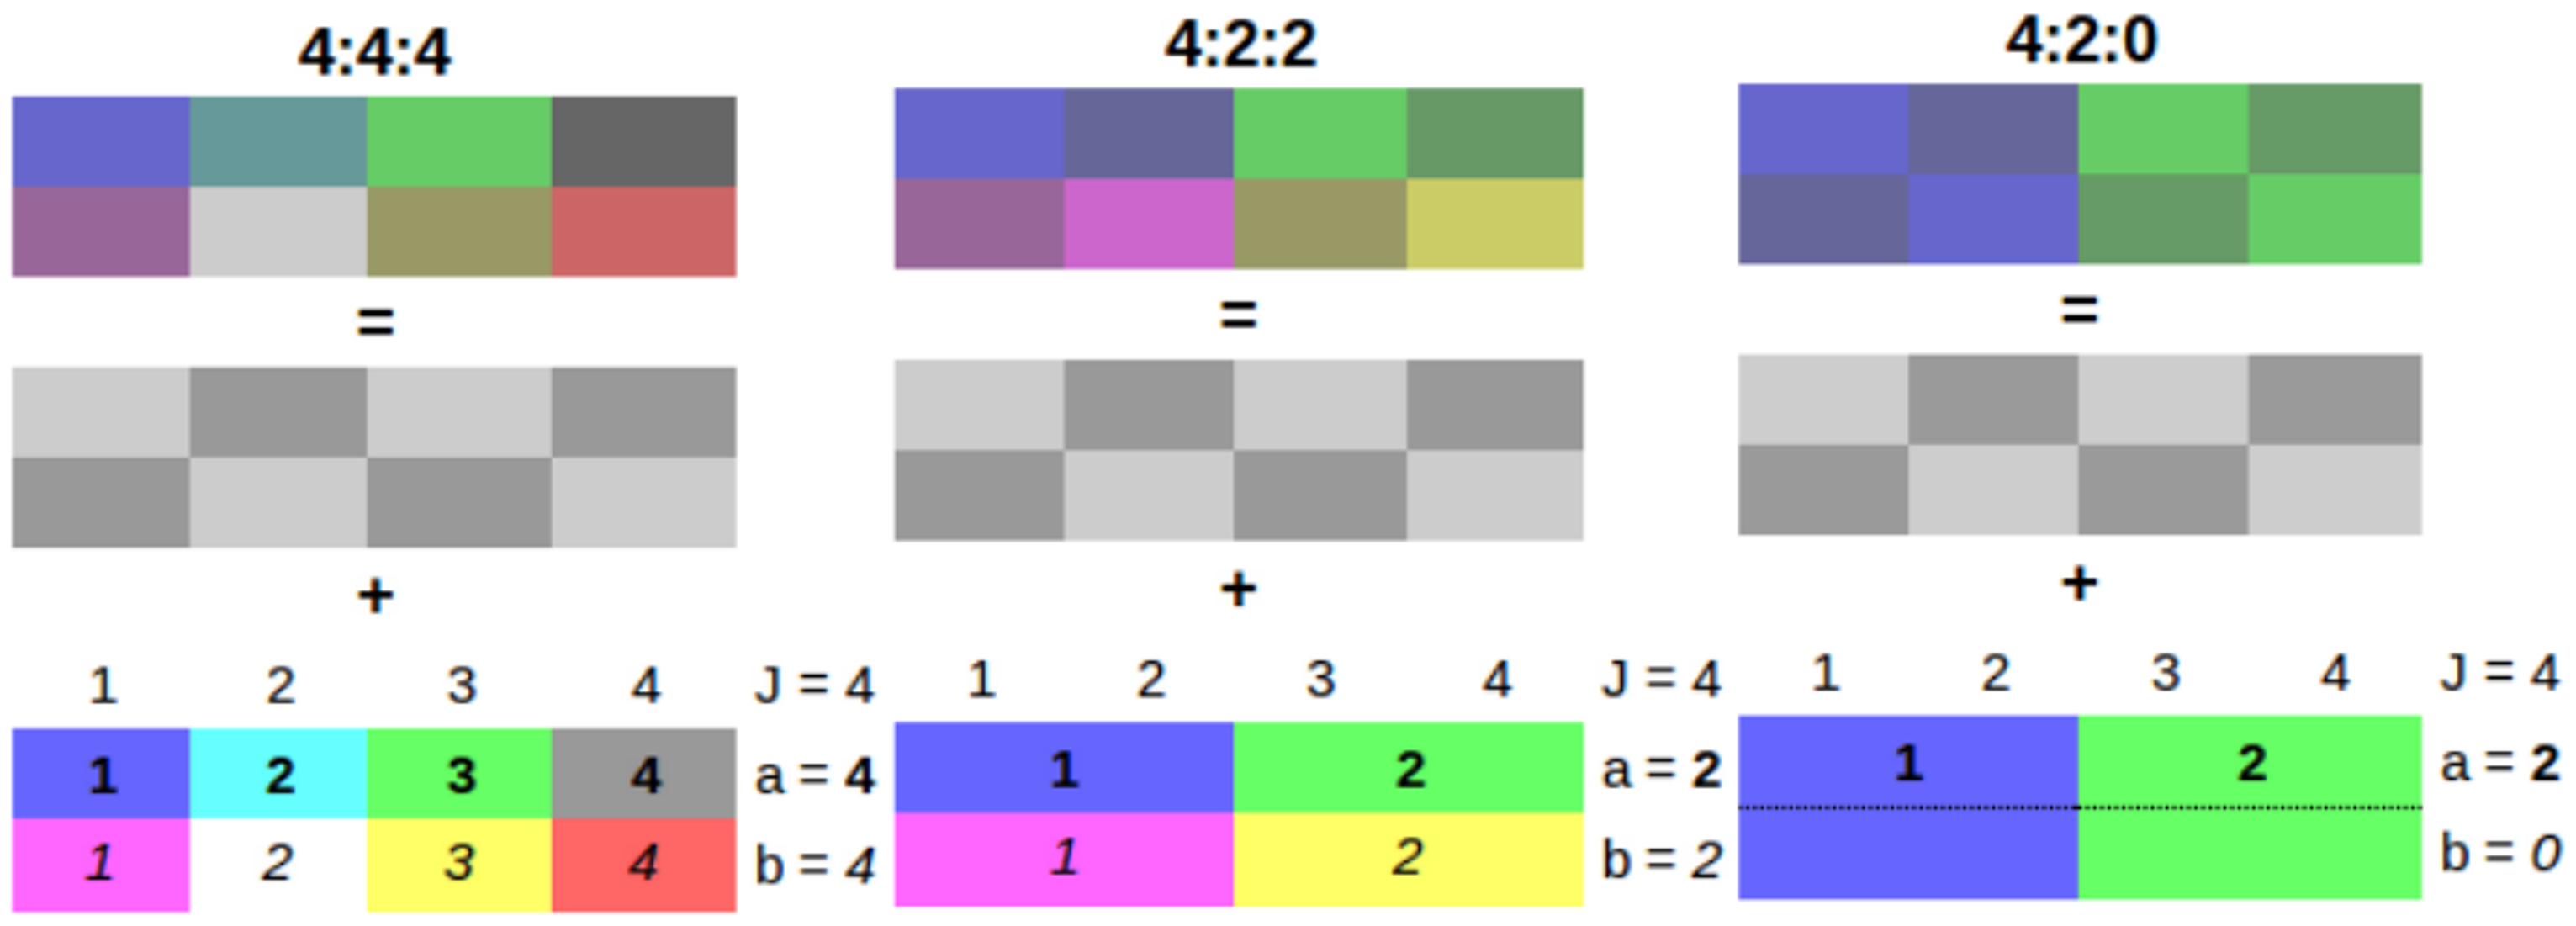
\includegraphics[width=1.0\textwidth]{pages/jpeg/chrominance_sample.png}
    \caption{3种色度采样示意}
    \label{Fig.chrominance_sample}
\end{figure}


\section{图像分块与DCT变换}
\subsection{图像分块}
\subsection{DCT变换}

一般的二维DCT变换
\begin{equation}
    \begin{aligned}
        F(u,v) &=c(u)c(v) \sum_{i=0}^{M-1} \sum_{j=0}^{N-1} f(i,j) \cos(\frac{i+0.5}{M}u\pi) \cos(\frac{j+0.5}{N}u\pi) \\
        c(u) &=\left\{\begin{aligned}
            & \sqrt{\frac{1}{N}}, & \quad u=0 \\
            & \sqrt{\frac{2}{N}}, & \quad u\neq 0
        \end{aligned}\right.
        \quad u,v=0,1,2,...,7
    \end{aligned}
\end{equation}
当 $M=N$ 时, DCT 变换可以表示为矩阵相乘的形式, $F$ 的 DCT 变换则是 $T=AFA^T$。变换矩阵 $A$ 为
\begin{equation}
    A=\frac{2}{\sqrt{N}}
    \begin{bmatrix}
        \frac{1}{\sqrt{2}}      & \frac{1}{\sqrt{2}}        & ...   & \frac{1}{\sqrt{2}} \\
        \cos\frac{\pi}{2N}      & \cos\frac{3\pi}{2N}       & ...   & \cos\frac{(2N-1)\pi}{2N} \\
        ...                     & ...                       &       & ... \\
        \cos\frac{(N-1)\pi}{2N} & \cos\frac{3(N-1)\pi}{2N}  & ...   & \cos\frac{(2N-1)(N-1)\pi}{2N}
    \end{bmatrix}
\end{equation}




当原始图像从 RGB 颜色空间转换到 YCbCr 颜色空间之后,需要对每一个 $8 \times 8$ 的图像块进行二维DCT变换
\begin{equation}
    \begin{aligned}
        F(u,v) &=c(u)c(v) \sum_{i=0}^{7} \sum_{j=0}^{7} f(i,j) \cos(\frac{i+0.5}{8}u\pi) \cos(\frac{j+0.5}{8}u\pi) \\
        c(u) &=\left\{\begin{aligned}
            & \sqrt{\frac{1}{8}},   & \quad u=0 \\
            & \frac{1}{2},          & \quad u\neq 0
        \end{aligned}\right.
        \quad u,v=0,1,2,...,7
    \end{aligned}
\end{equation}

这时候的 DCT 变换矩阵为
\begin{equation}
    A=\frac{1}{\sqrt{2}}
    \begin{bmatrix}
        \frac{1}{\sqrt{2}}      & \frac{1}{\sqrt{2}}        & ...   & \frac{1}{\sqrt{2}} \\
        \cos\frac{\pi}{16}      & \cos\frac{3\pi}{16}       & ...   & \cos\frac{(16-1)\pi}{16} \\
        ...                     & ...                       &       & ... \\
        \cos\frac{(N-1)\pi}{16} & \cos\frac{3(N-1)\pi}{16}  & ...   & \cos\frac{(16-1)(N-1)\pi}{16}
    \end{bmatrix}
\end{equation}

在 Matlab 中可以用 \lstinline|T = dctmtx(8)| 查看
\begin{lstlisting}{Matlab}
T =
  0.3536  0.3536  0.3536  0.3536  0.3536  0.3536  0.3536  0.3536
  0.4904  0.4157  0.2778  0.0975 -0.0975 -0.2778 -0.4157 -0.4904
  0.4619  0.1913 -0.1913 -0.4619 -0.4619 -0.1913  0.1913  0.4619
  0.4157 -0.0975 -0.4904 -0.2778  0.2778  0.4904  0.0975 -0.4157
  0.3536 -0.3536 -0.3536  0.3536  0.3536 -0.3536 -0.3536  0.3536
  0.2778 -0.4904  0.0975  0.4157 -0.4157 -0.0975  0.4904 -0.2778
  0.1913 -0.4619  0.4619 -0.1913 -0.1913  0.4619 -0.4619  0.1913
  0.0975 -0.2778  0.4157 -0.4904  0.4904 -0.4157  0.2778 -0.0975
\end{lstlisting}

对图像进行 $8\times 8$ 分块后,对每一个矩阵块 A 都进行 DCT 变换 $TAT^T$ 

\section{量化}
\section{熵编码}
\subsection{霍夫曼编码}
霍夫曼编码是一种用于无损数据压缩的熵编码(权编码)算法,其使用变长编码表对数据进行编码。

变长编码表是通过评估符号出现概率得到的,出现概率高的符合使用较短的编码,反之出现概率低的则使用较长的编码,使编码之后的字符串的平均长度降低,从而达到无损压缩数据的目的。

霍夫曼编码主要分为两步:

根据每个字符出现的概率构建一颗最优二叉树;

再根据二叉树对字符进行编码。
